\label{sec:vbf-evtsel}

The event selection targets two different signal topologies:
\begin{itemize}
\item \fourcentral: both VBF jets and \bjets from the Higgs decay are 
  found in the central region of the detector ($|\eta|<2.8$)
\item \twocentral: at least one VBF jet is required to be
  in the forward region ($|\eta|>3.1$)
\end{itemize}

These two categories are designed to be exclusive and are fed by two separate trigger paths.  

\subsubsection{Trigger Definitions}

\paragraph{\fourcentral:} Two triggers are used for this channel depending on the data taking periods. The first dataset (data taking periods A-D of year 2016) uses HLT\_2j45\_bmv2c2070\_split\_2j45, which requires four central Level-1 jet objects, referred to as regions of interest (ROI),  with \ET $>$ 15 \GeV~( L1\_4J15).  In the HLT, two of these jets are required to have an HLT jet \ET of at least 45 \GeV~and be tagged with the 70\% working point of online $b$-tagging algorithm. The integrated luminosity of this first trigger is 9.4~\ifb. In the second dataset (data taking periods E-L) due to the bandwidth limit imposed by increasing luminosity, this analysis switched to using the HLT\_2J35\_bmv2c60\_2J35 trigger, which is seeded by the same L1 object.  In the HLT two of these jets are required to have an HLT jet \ET of at least 35 \GeV~and be tagged with the 60\% working point of online $b$-tagging algorithm. The integrated luminosity of this trigger is 13.3~\ifb.

\paragraph{\twocentral:} The HLT\_j80\_bmv2c2070\_split\_j60\_bmv2c2085\_split\_j45\_320eta490 is used for this channel for the entire dataset.  At L1, it requires at least one central jet with a Level-1 ROI \ET of 40 \GeV~and $|\eta| < 2.5$.  Additionally it requires another central jet with ROI \ET $>$ 25 \GeV~and a third, forward jet with ROI \ET of at least 20 and  $3.1 < |\eta| < 4.9$.   At the HLT one central jet \btagged  with the 70\% online working point and at least 80 \GeV~is required, in addition to a second jet with at least 60 \GeV~tagged at the looser 85\% working point. Lastly, the forward jet is required to have \ET $>$ 45 \GeV~at the HLT.


\subsubsection{Event Pre-Selection and Jet Assignment}
\label{sec:vbf-presel}

\paragraph{\fourcentral:} Events are required to pass the \fourcentral trigger depending on the data taking period. At least two offline jets with \pT $>$ 55 \GeV~and ($|\eta| < 2.5$) which pass the offline \btagging at the medium working point are required for the event to pass pre-selection.  These jets also have to be matched to the HLT trigger \btagged trigger objects. Two additional jets with \pT $>$ 55 \GeV~and  ($|\eta| < 2.8$) are also required. If there is a jet with \pT $>$ 60 \GeV~and 3.2 $< |\eta| <$ 4.4 the event is vetoed in order to avoid overlap with the \twocentral channel.

All pairs of \btagged jets passing the medium working point are considered and the highest \pT  pair becomes our Higgs candidate.  All pairs of non-\btagged jets are also considered and the highest invariant mass pair form the VBF jets. Events in which the VBF jets pair cannot be formed are rejected.
%The VBF jet assignment fails where there are only four jets above the \pT threshold, of which three are $b$-tagged.
%These events are rejected. 

%Lastly, only events with a Higgs candidate transverse momentum, \pTbb, %of 
%greater than 150 \GeV~are considered.  This requirement is needed to remove kinematic sculpting of the \Mbb distribution in the low \Mbb region.  Figure~\ref{fig:mbb_ptcuts} shows the \Mbb distribution for a variety of \pTbb cuts for the  pre-selected events outside of the Higgs mass window (the background sample) for the \fourcentral channel on the left.  It can be seen that a broad ``bump" is present in the distribution between 200 and 300~\GeV~when no \pTbb cuts are applied.  

\paragraph{\twocentral:} Events are required to pass HLT\_j80\_bmv2c2070\_split\_j60\_bmv2c2085\_split\_j45\_320eta490.   We require at least one offline jet with \pT $>$ 95 \GeV~which is \btagged at the medium working point.  We also require at least one additional jet with \pT $>$ 70 \GeV~which passes the loose offline \btagging working point.  These two jets must be matched to the HLT \btagged objects.  In addition to these jets, at least one forward jet with \pT $>$ 60 \GeV~and 3.2 $< |\eta| <$ 4.4 is required.  Lastly, the event must have at least one more jet with \pT $>$ 20 \GeV~ and $|\eta| <$ 4.4.  

Jet assignment proceeds as follows.  All pairs of \btagged jets passing the loose working point which contain at least one jet passing the medium working point are considered and the highest \pT pair becomes our Higgs candidate.  The VBF jet candidates are formed from all pairs of jets passing pre-selection which are not part of the Higgs candidate pair,  including at least one of the forward jets from the pre-selection.  There is no requirement that these jets fail  the \btagging requirements. The highest invariant mass pair are labeled the VBF jets. 

%Lastly, only events with a Higgs candidate transverse momentum, \pTbb, greater than 160 \GeV~are considered.  This requirement is needed to remove kinematic sculpting of the \Mbb{} distribution in the low \Mbb{} region.  \Mbb{} is correlated with \pTbb{}, and the \pTbb{} distribution has a turn-on due to the jet \pT requirements. Figure~\ref{fig:mbb_ptcuts} shows the \Mbb distribution for a variety of \pTbb cuts for the background sample for the \twocentral channel on the right.  As the \pTbb{} cut is increased, the distribution assumes a regular falling spectrum.  The sculpting is worse for the \twocentral channel than the \fourcentral channel due to the higher threshold jet requirements.


\paragraph{\pTbb cut:} Common to both channels is a \pTbb cut applied at the last step of pre-selection. This cut effectively is a also a cut on the \pT of both \bjets. As shown in Fig. \ref{fig:vbf-mbb_ptcuts}, the jet trigger and kinematic requirements sculpt the \Mbb distribution. A \pTbb cut at 150\GeV and 160\GeV is applied to \fourcentral and \twocentral channels smooth the \Mbb distribution.

\begin{figure}[htbp]
  \centering
 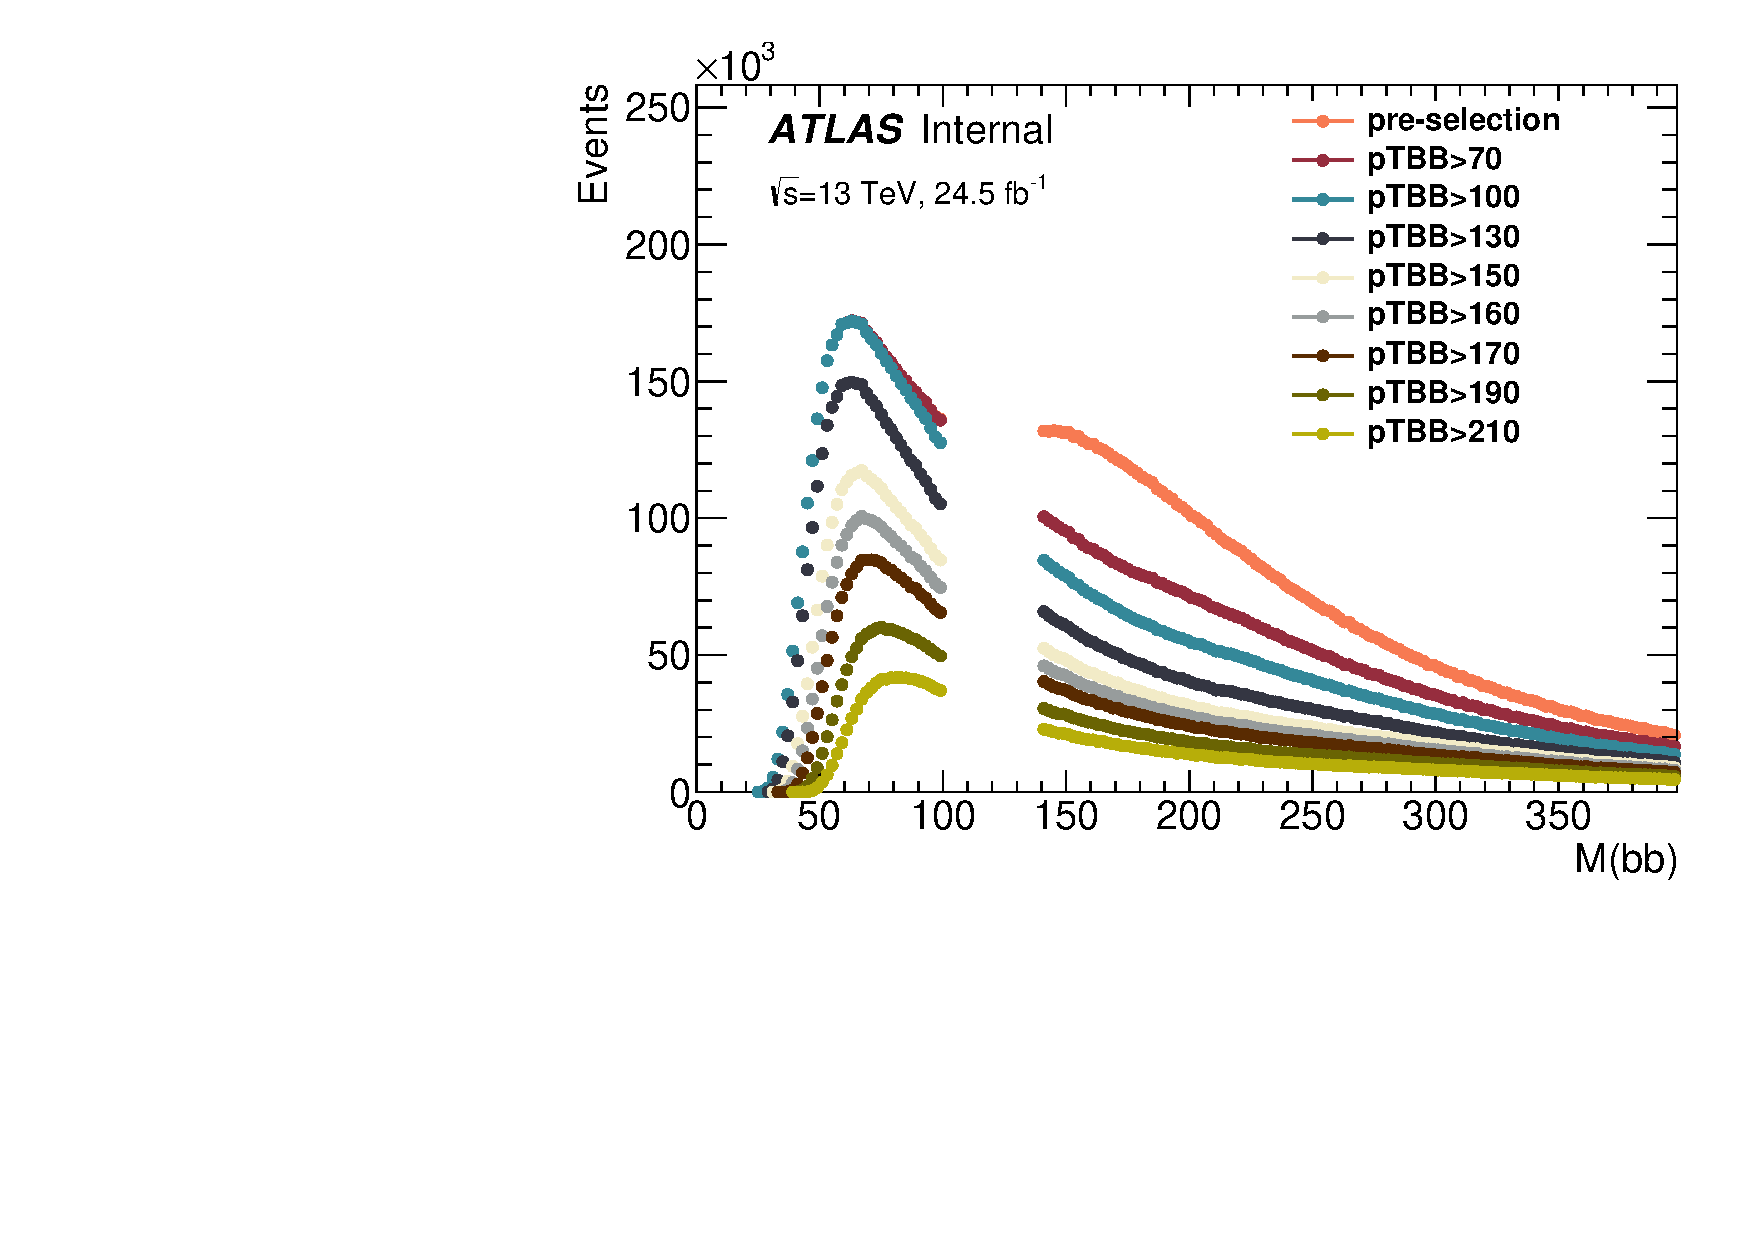
\includegraphics[width=0.45\textwidth]{figures/VBF/Presel-Mbb_4cen.pdf}
 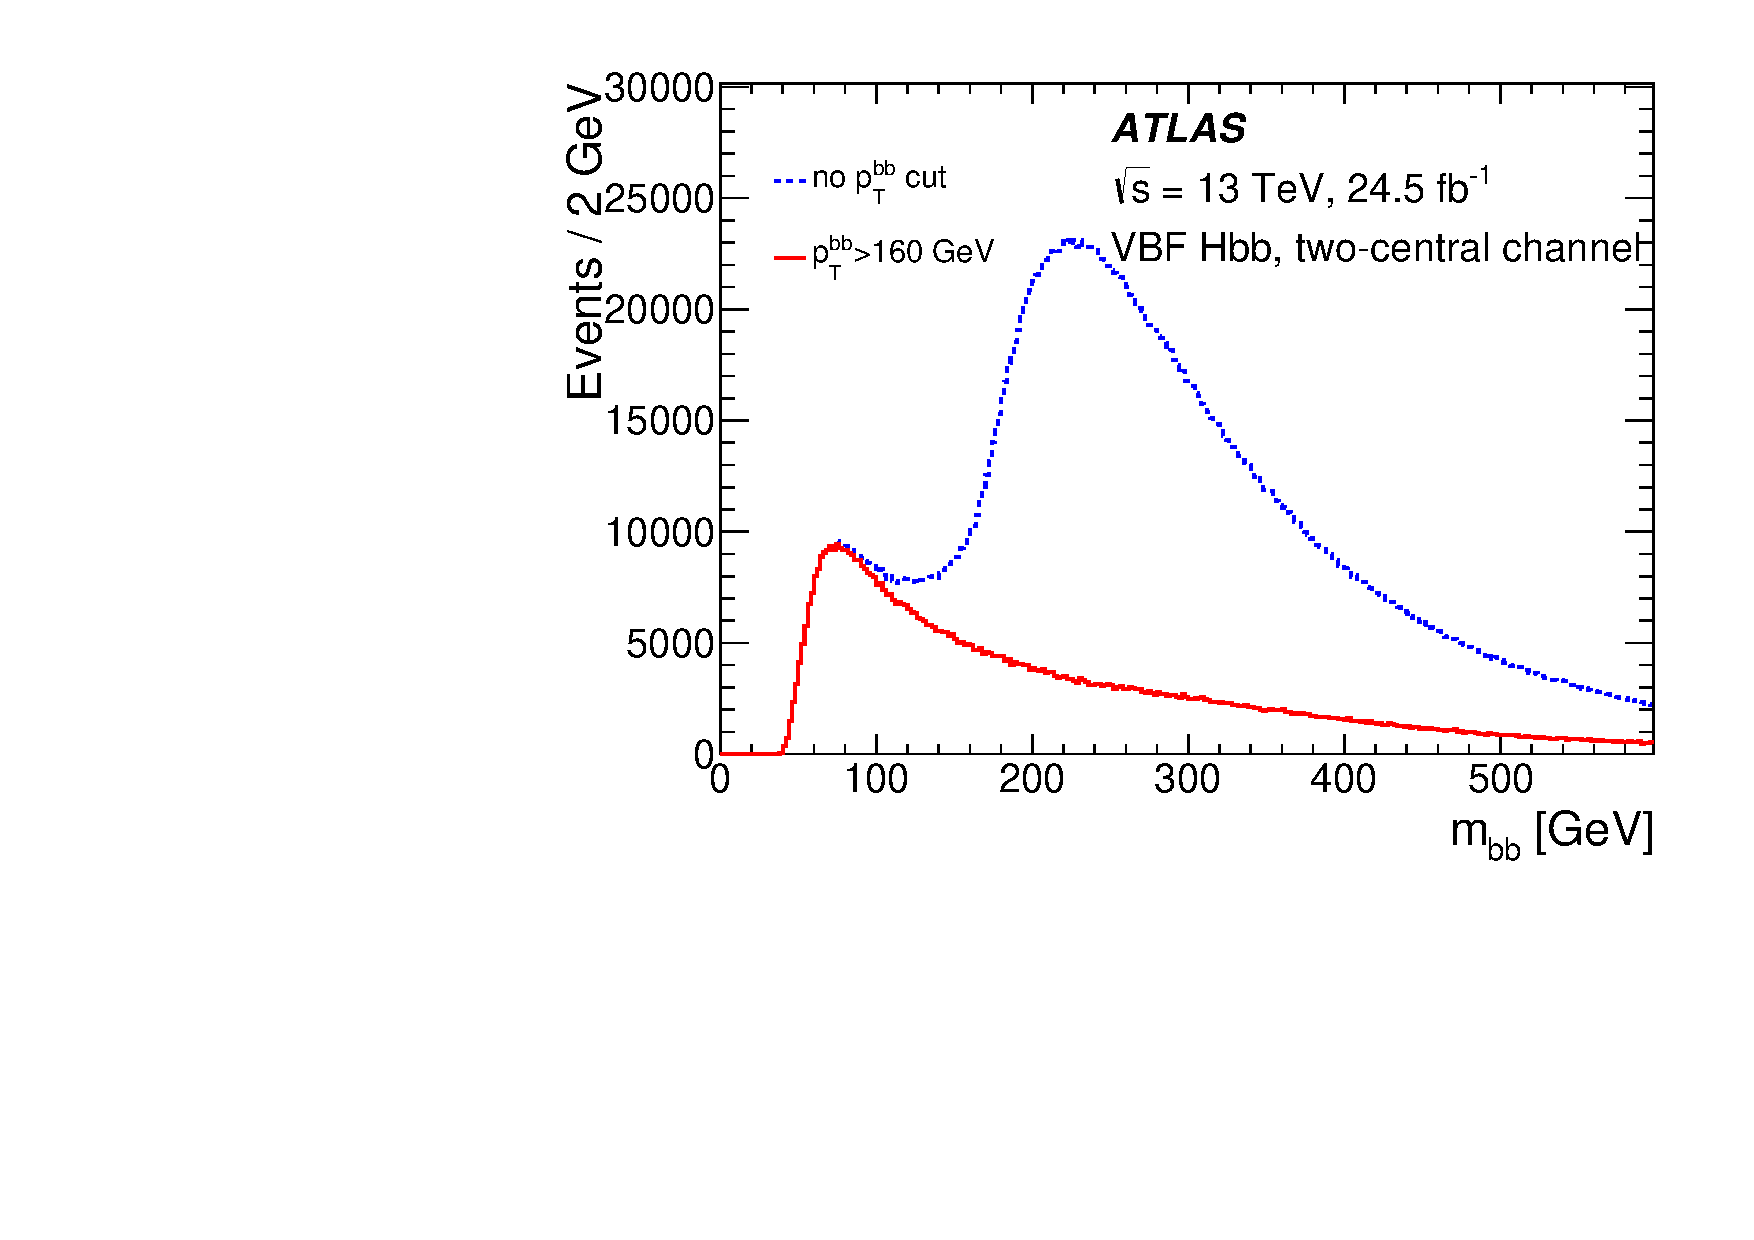
\includegraphics[width=0.45\textwidth]{figures/VBF/Presel-Mbb_2cen.pdf}
 \caption{Distributions of \Mbb for a variety of \pTbb cuts using data events.  \fourcentral events on the left, \twocentral on the right.  All event pre-selection criteria except the \pTbb cuts are applied.}
  \label{fig:vbf-mbb_ptcuts}
\end{figure}


%\paragraph{0-tag samples:} Both the \fourcentral and \twocentral channels have corresponding 0-tag samples in which the offline jets are required to be anti-\btagged at the 85\% working point. These samples are used to determine the sensitivity when determining the signal and control BDT regions.   A relatively tight anti-tag is required in order to minimize any leakage of the signal into the 0-tag sample.  In these samples supporting triggers are used, which have the same Level-1 and HLT jet requirements, but no \btagging requirements.  These triggers are heavily pre-scaled.  

\paragraph{Overlap with VBF$+\gamma$ Analysis:} The result of this analysis is eventually combined with the complementary VBF$+\gamma$ analysis which studies the same event topology with an additional photon radiated by the initial/final state quarks or the vector bosons. For the two analyses to remain orthogonal, the inclusive analysis vetoes events selected by the VBF$+\gamma$ analysis in data. From simulation it is determined that only 0.11\% and 0.047\% of the inclusive VBF signal MC would pass selections of both analyses given that they pass \twocentral and \fourcentral respectively. The size of this overlap is so small, less than $0.5\%$ (a criterion for us to account a particular source of systematics in the final fit \ref{sec:vbf-uncertainties}), such that it is neglected.  

%Then put into BDT & we have SR1, SR2 & CR.  Used to have 0 tag control sample but not used.
%The details of the event selection are summarized in Table~\ref{tab:evtsel}. 
%With exception of the trigger requirements, the same requirements are placed on the data and MC samples.  In the MC15 samples the trigger decision is missing for the \twocentral channel, therefore an alternative emulation is used, described briefly in Section~\ref{sec:vbf-trig}.


The details of the event selection are summarized in Table~\ref{tab:evtsel}. Cut flows for both selections are displayed in Tables~\ref{tab:cutflow_4cen} and~\ref{tab:cutflow_2cen}.


\begin{table}[htbp]
  \begin{center}
    \resizebox{\textwidth}{!}{
      \begin{tabular}{ l  c c }
        \toprule
        & \fourcentral & \twocentral \\
        \midrule
        L1 trigger          & L1\_4J15                 & L1\_J40\_0ETA25\_2J25\_J20\_31ETA49                                \\
\\
        Primary HLT trigger  & HLT\_2j45\_bmv2c2070\_split\_2j45  & HLT\_j80\_bmv2c2070\_split\_j60\_bmv2c2085\_split\_j45\_320eta490  \\ 
                 & HLT\_2j35\_bmv2c2060\_split\_2j35  &   \\ 

      \\ 
        Support HLT trigger & HLT\_4j45                          & HLT\_j80\_0eta240\_j60\_j45\_320eta490                             \\ 
        \\
                                              &                                                     & $\geq4$ jets with $\pt>20$ \GeV{} and $|\eta|<4.4$ \\
                                              &                                                     & $\geq1$ jet with $\pt>60$ \GeV{} and $3.2<|\eta|<4.4$  \\ 
                                              &                                                     & $\geq2$ jets with $\pt>70$ \GeV{} and $|\eta|<2.5$ \\ 
        \multirow{-4}{*}{Jet selection}       & \multirow{-4}{*}{$\geq4$ jets with $\pt>55$ \GeV{} and $|\eta|<2.8$} & $\geq1$ jet with $\pt>95$ \GeV{} and $|\eta|<2.4$  \\ 
        \\
        
        \multirow{2}{*}{$b$-tagging}          & \multirow{2}{*}{$\geq2$ $b$-jets with $\pt>55$ \GeV{} and $|\eta|<2.5$} & $\geq2$ $b$-jets with $\pt>70$ \GeV{}                  \\ 
                                              &                                                        & $\geq1$ $b$-jets with $\pt>95$ \GeV{} and $|\eta|<2.4$ \\ 
        Forward jet veto                      &   No jet with $\pt>60$ \GeV{} and $3.2<|\eta|<4.4$    &  \\ 
        Higgs boson candidate                 &       $\pt(b\bar{b})>150$ \GeV{}                       &  $\pt(b\bar{b})>160$ \GeV{} \\  
        
        \bottomrule
      \end{tabular}
    }
  \end{center}
  \caption{Event selection for the two event categories. The \fourcentral has two primary trigger paths.  The first is used for the pre-ICHEP dataset, the second is used for the post-ICEP dataset. \bjets{} are tagged with the 70\% working point and are required to have $|\eta| < 2.5$}
  \label{tab:evtsel}
\end{table}




\begin{table}[]
\centering

\begin{tabular}{|l|l|l|l|l|l|}
\hline
                       & \multicolumn{5}{c|}{Pre-ICHEP}                                 \\ \hline
                       & data 2tag  & VBF       & ggF        & Zbb(QCD)     & Zbb(EWK)  \\ \hline
Events                 & 122517049* & 20127.8 & 234762.8 & 3880727.1    & 29277.8 \\ \hline
Trigger                & 29623250   & 627.0    & 2192.1    & 98931.1    & 1444.5  \\ \hline
2 medium \btagged jets & 13910362   & 334.3    & 1207.3    & 45110.5    & 705.0    \\ \hline
$\ge$ 4 jets           & 9255271    & 215.2    & 892.1     & 35903.9    & 566.7    \\ \hline
Forward jet veto       & 9021208    & 205.8    & 869.9     & 34675.7    & 545.1    \\ \hline
Jet Assignment         & 8290467    & 197.2    & 820.2     & 33604.2    & 532.1    \\ \hline
$\pTbb>150\GeV$        & 3146579    & 121.8    & 532.4     & 21084.0    & 379.2    \\ \hline
Photon veto in data    & 3145966    & 121.8    & 532.4     & 21084.0    & 379.2    \\ \hline
                       & \multicolumn{5}{c|}{Post-ICHEP}                                \\ \hline
                       & data 2tag  & VBF       & ggF        & Zbb(QCD)     & Zbb(EWK)  \\ \hline
Events                 & 169139398* & 28565.5 & 332929.0 & 5505804.9 & 41551.4 \\ \hline
Trigger                & 43820814   & 1024.1   & 3602.9    & 166327.2   & 2271.5  \\ \hline
2 medium \btagged jets & 19370468   & 501.8    & 1868.4    & 64549.5    & 955.6    \\ \hline
$\ge$ 4 jets           & 10218887   & 273.8    & 1133.7    & 45143.9    & 712.8    \\ \hline
Forward jet veto       & 9963404    & 261.9    & 1105.7    & 43605.2    & 685.1    \\ \hline
Jet Assignment         & 9065632    & 250.2    & 1037.5    & 42163.0    & 667.9    \\ \hline
$\pTbb>150\GeV$        & 3755031    & 158.0    & 685.4     & 27202.8    & 486.5    \\ \hline
Photon veto in data    & 3754301    & 158.0    & 685.4     & 27202.8    & 486.5    \\ \hline
\end{tabular}
  \caption{Cutflow for the \fourcentral events.  MC events are normalized to cross section times branching ratio.  The total number of data events is after the application of the derivation skimming whereas the MC events are the total number of events in the MC samples scaled to the luminosity of the corresponding datasets (9.4\ifb and 13.3\ifb for first and second datasets respectively).}
  \label{tab:cutflow_4cen}
\end{table}


\begin{table}[]
\centering
  
\begin{tabular}{|l|l|l|l|l|l|}
\hline
                            & data       & VBF       & ggF       & Zbb(QCD)    & Zbb(EWK)    \\ \hline
Events                      & 291656447* & 52628.6 & 613382.5 & 10143797.6 & 76540.4    \\ \hline
Trigger                     & 18425823   & 679.2    & 594.0    & 23942.1    & 555.7      \\ \hline
1 Medium \btagged jet       & 10321971   & 455.0    & 405.2    & 14816.1    & 369.6      \\ \hline
$\ge$ 2 loose \btagged jets & 3529025    & 269.7    & 244.5    & 7753.0     & 203.9      \\ \hline
Forward jet requirement     & 2814936    & 214.9    & 181.6    & 5328.1     & 162.7      \\ \hline
$\ge$ 4 jets                & 2527300    & 208.1    & 176.0    & 5307.6     & 161.7      \\ \hline
Jet Assignment              & 2527300    & 208.1    & 176.0    & 5307.6     & 161.7      \\ \hline
$\pTbb>160\GeV$             & 884095     & 147.3    & 126.5    & 3565.7     & 122.4      \\ \hline
Photon veto in data         & 883906     & 147.3    & 126.5    & 3565.7     & 122.4      \\ \hline
\end{tabular}
   \caption{Cutflow for the \twocentral events. MC events are normalized to cross section times branching ratio. The total number of data events is after the application of the derivation skimming whereas the MC events are the total number of events in the MC samples scaled to the total luminosity (24.5\ifb). *The data number of total events is the number of all events after the derivation skim.}
   \label{tab:cutflow_2cen}
\end{table}

